\documentclass{article}

\usepackage[pdftex]{graphicx}
\usepackage[czech]{babel}
\usepackage[utf8]{inputenc}
\usepackage{enumitem}
\usepackage{amsmath}
\usepackage{url}
\usepackage{listings}
\usepackage{caption}
\usepackage{gensymb}
\usepackage[usenames,dvipsnames,svgnames,table]{xcolor}

\usepackage[pdftex]{hyperref}
\hypersetup{colorlinks=true,
  unicode=true,
  linkcolor=black,
  citecolor=black,
  urlcolor=black,
  bookmarksopen=true}

\usepackage{xcolor}
\colorlet{mygray}{black!30}
\colorlet{mygreen}{green!60!blue}
\colorlet{mymauve}{red!60!blue}
\lstset{
	backgroundcolor=\color{gray!10},  
	basicstyle=\ttfamily,
	columns=fullflexible,
	breakatwhitespace=false,      
	breaklines=true,                
	captionpos=b,                    
	commentstyle=\color{mygreen}, 
	extendedchars=true,              
	frame=single,                   
	keepspaces=true,             
	keywordstyle=\color{blue},      
	language=c++,                 
	numbers=none,                
	numbersep=5pt,                   
	numberstyle=\tiny\color{blue}, 
	rulecolor=\color{mygray},        
	showspaces=false,               
	showtabs=false,                 
	stepnumber=5,                  
	stringstyle=\color{mymauve},    
	tabsize=3,                      
	title=\lstname                
}

\usepackage[numbers,sort&compress]{natbib}

\newcommand*\justify{
  \fontdimen2\font=0.4em
  \fontdimen3\font=0.2em
  \fontdimen4\font=0.1em
  \fontdimen7\font=0.1em
  \hyphenchar\font=`\-
}

\makeatletter
\def\subtitle#1{\gdef\@subtitle{#1}}
\def\maketitle{\begin{titlepage}%
		\let\footnotesize\small
		\let\footnoterule\relax
		\let \footnote \thanks
		\null\vfil
		\vskip 60\p@
		\begin{center}%
			{\LARGE \@title \par}%
			\vskip 1.5em% Added this
			{\Large \@subtitle \par}% and this
			\vskip 3em%
			{\large
				\lineskip .75em%
				\begin{tabular}[t]{c}%
					\@author
				\end{tabular}\par}%
			\vskip 1.5em%
			{\large \@date \par}%       % Set date in \large size.
		\end{center}\par
		\@thanks
		\vfil\null
	\end{titlepage}%
	\setcounter{footnote}{0}%
	\global\let\thanks\relax
	\global\let\maketitle\relax
	\global\let\@thanks\@empty
	\global\let\@author\@empty
	\global\let\@date\@empty
	\global\let\@title\@empty
	\global\let\title\relax
	\global\let\author\relax
	\global\let\date\relax
	\global\let\and\relax
}
\makeatother

% NASTAVENI JAZYKA: #1 pro CZ, #2 pro EN
\newcommand\lang[2]{#1}

\title{KIV-DPP-01}
\subtitle{\lang{Dokumentace rozšiřující desky}{Expansion board documentation}}
\author{Martin Úbl}
\date{\lang{1. září 2021}{1 September 2021}}

\begin{document}

\maketitle



\section{\lang{Přehled}{Overview}}

\begin{figure}[ht]
	\centering
	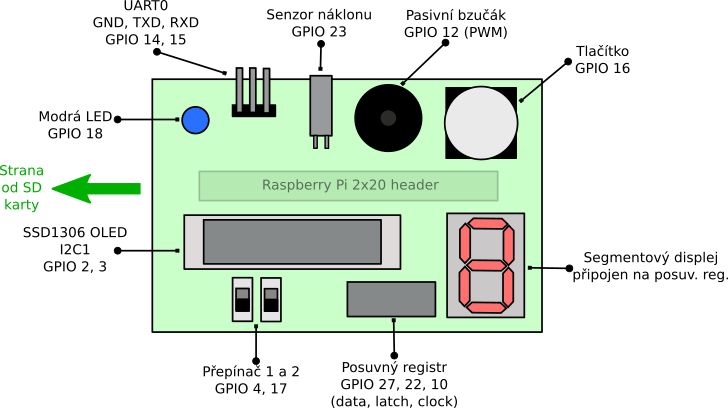
\includegraphics[width=1.0\linewidth]{kiv-dpp-01.png}
\end{figure}

\lang{Deska KIV-DPP-01 (KIV Deska Plná Periferií rev. 01) obsahuje následující sadu periferií:}{The KIV-DPP-01 expansion board houses the following set of peripherals:}
\begin{itemize}
	\item \lang{Modrá}{Blue} LED (GPIO 18)
	\item UART header (GPIO 14, 15)
	\item \lang{Senzor náklonu}{Tilt sensor} (GPIO 23)
	\item \lang{Pasivní bzučák}{Passive buzzer} (GPIO 12)
	\item \lang{Tlačítko}{Push button} (GPIO 16)
	\item \lang{Sedmi-segmentový displej (přímo připojen na posuvný registr)}{7-segment display (directly connected to the shift register)}
	\item \lang{Posuvný registr}{Shift register} 74HC595N (GPIO 27, 22, 10)
	\item \lang{Polohový přepínač}{Switch} 1 (GPIO 4)
	\item \lang{Polohový přepínač}{Switch} 2 (GPIO 17)
	\item SSD1306 OLED \lang{displej}{display} (I2C1; GPIO 2, 3)
\end{itemize}

\newpage

\section{\lang{Zapojení}{Connection}}

\lang{Deska obsahuje 2x20-pin header, který přímo pasuje do pinového protikusu na straně Raspberry Pi. Důležité je dodržet orientaci rozšiřující desky vůči Raspberry Pi -- LED na rozšiřující desce se musí nacházet na straně, kde se na hostitelské desce nachází slot na SD kartu. Posuvný registr a segmentový displej se pak nachází na straně, kde má hostitelská deska umístěné USB konektory.
}
{
The board contains 2x20-pin F header, which is intended to be directly connected to M header on the Raspberry Pi side. It is important to rotate the board correctly -- LED on the expansion board must be on the same side, as the SD card slot on the host board. The shift register and segment display is then localized on the same side, as USB ports on the host board.
}

\section{LED}

\begin{itemize}
	\item \lang{Barva: modrá}{Color: blue} (455-465 nm)
	\item GPIO: 18
	\item \lang{Zapojení}{Wiring}: IN - LED - GND
	\item \lang{Spotřeba}{Current}: max. 20 mA
	\item \lang{Svítivost}{Luminosity}: max. 3000 mcd
\end{itemize}

\lang{Klasická modrá LED, anoda je vyvedená na GPIO pin 18, katoda na GND.}{Standard blue LED, anode is connected to GPIO 18, cathode is connected to GND.}

\section{UART header}

\begin{itemize}
	\item GPIO: 14 (TXD), 15 (RXD)
	\item \lang{Zapojení: přímé}{Wiring: direct}
\end{itemize}

\lang{Header pro připojení UART terminálu, např. USB-TTL převodník do hostitelského PC. Piny jsou zleva (od LED) zapojeny na: GND, TXD, RDX. Zapojení je přímé -- do hostitelského počítače tedy musí být překřížené.}
{Header for UART terminal connection, e.g. the USB-TTL converter to host PC. Pins are connected (from left to right) to: GND, TXD, RXD. The wiring is direct -- wiring should be crossed over to the other end.}

\section{\lang{Senzor náklonu}{Tilt sensor}}

\begin{itemize}
	\item GPIO: 23
	\item \lang{Zapojení}{Wiring}: pull-up
	\item Datasheet: \url{http://home.zcu.cz/~ublm/files/os/SW-520D.pdf}
\end{itemize}

\lang{Kuličkový senzor náklonu SW-520D, který je připájený úmyslně pod úhlem cca 15\degree, dovede detekovat, zda je zařízení v horizontální nebo vertikální poloze (resp. \uv{půl-poloze} vzhledem k povaze senzoru).}
{Ball tilt sensor SW-520D, which is soldered to the expansion board under 15\degree angle. This sensor is able to sense, if the device is in horizontal or vertical position (or \uv{half-position} due to the sensor type).}

\section{\lang{Pasivní bzučák}{Passive buzzer}}

\begin{itemize}
	\item GPIO: 12
	\item \lang{Zapojení: přímé}{Wiring: direct}
	\item \lang{Odpor}{Resistance}: 16 $\Omega$
\end{itemize}

\lang{Pasivní bzučák zapojený na GPIO 12. Bzučák je pasivní, takže nemá interní oscilátor -- je nutné ho tedy řídit PWM signálem.}{Passive buzzer connected to GPIO 12. The buzzer is passive, so it does not have the internal oscilator -- the pulse-width modulation (PWM) is needed to drive the buzzer.}

\section{\lang{Tlačítko}{Push button}}

\begin{itemize}
	\item GPIO: 16
	\item \lang{Zapojení: pull-up}{Wiring: pull-up}
\end{itemize}

\lang{Klasické tlačítko s plastovou čepičkou.}{Standard push button with plastic cap.}

\section{\lang{Sedmi-segmentový displej}{7-segment display}}

\begin{itemize}
	\item GPIO: -
	\item \lang{Zapojení: společná katoda}{Wiring: common cathode}, IN - LED - 3.3V
	\item \lang{Spotřeba}{Current}: max. 15 mA
	\item Datasheet: \url{http://home.zcu.cz/~ublm/files/os/5161AS.pdf}
\end{itemize}

\lang{Sedmi-segmentový displej 5161AS je připojený na výstupy posuvného registru. Nelze jej tedy ovládat samostatně. Zapojení je se společnou katodou.}{7-segment display 5161AS is connected directly to the outputs of the shift register. It's not possible to control it directly. It is wired with common cathode.}

\lang{Zobrazovací jednotka je na výstupy posuvného registru připojena následovně:}{The display is connected to the shift register as follows:}
\begin{figure}[ht!]
	\centering
	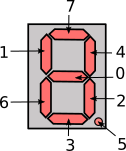
\includegraphics[width=0.3\linewidth]{kiv-dpp-01-segments.png}
\end{figure}

\section{\lang{Posuvný registr}{Shift register}}

\begin{itemize}
	\item GPIO: 27 (data), 22 (latch), 10 (clock)
	\item \lang{Zapojení: přímé}{Wiring: direct}
	\item Datasheet: \url{http://home.zcu.cz/~ublm/files/os/74HC565.pdf}
\end{itemize}

\lang{Posuvný registr 74HC595N je vstupy zapojen přímo na GPIO 27 (datový pin), 22 (latch pin, přepnutí banku) a 10 (časovací signál). Výstupy jsou zapojeny na vstupy sedmi-segmentového displeje.}{The shift register 74HC595N is connected to GPIO 27 (data pin), 22 (latch pin, bank shift) and 10 (timing signal). Outputs are connected to inputs of the 7-segment display.}

\section{\lang{Polohové přepínače}{Switches}}

\begin{itemize}
	\item GPIO: 4 (\lang{př.}{sw.} 1), 17 (\lang{př.}{sw.} 2)
	\item Zapojení: pull-down
\end{itemize}

\lang{Běžné malé nezávisle zapojené polohové přepínače.}{Common switches, connected independently.}

\section{OLED \lang{displej}{display}}

\begin{itemize}
	\item I2C: \lang{kanál}{channel} 1
	\item GPIO: 2 (SDA), 3 (SCL)
	\item \lang{Zapojení: přímé}{Wiring: direct}
	\item \lang{Typ: monochromatický (modrá nebo bílá)}{Type: monochromatic (blue or white)}
	\item \lang{Velikost matice: 128x32 bodů}{Matrix size: 128x32 pixels}
	\item Datasheet: \url{http://home.zcu.cz/~ublm/files/os/SSD1306.pdf}
\end{itemize}

\lang{Displej SSD1306 je přímo připojený na piny 2 a 3, na kterých na hostitelské desce operuje I2C kanál 1. Protokol pro ovládání displeje je shodný pro všechny displeje z řady SSD1306 (všechny rozměry). Body displeje mohou svítit buď bílou nebo modrou barvou.}
{The SSD1306 display is directly connected to pins 2 and 3, on which the host board operates I2C channel 1. The protocol is common for all SSD1306 displays (all variants and dimensions). Pixels glow either blue or white.}

\end{document}























